\section{Apprentissage artificiel}

\subsection{Présentation générale}

% \comment{}{Présentation plus générale s'inspirant de http://fr.wikipedia.org/wiki/Apprentissage_supervis\%C3\%A9. Note qu'il existe aussi un apprentissage non-supervisé qu'on ignore ici.}

D'un point de vue informatique, un algorithme d'apprentissage peut être vu comme un objet doté de 2 types de paramètres:
\begin{itemize}
 \item des paramètres dépendant des données, notés $\theta$, qu'on va estimer à partir de données d'apprentissage
 \item des paramètres fixés à la création de l'objet appelés hyper-paramètres
\end{itemize}
Son utilisation se fait en 2 phases:
\begin{itemize}
 \item une phase d'apprentissage (voir~\autoref{fig:Apprentissage_Machine}) au cours de laquelle on va estimer les paramètres $\theta$ grâce à 2 jeux de données:
 une matrice $X_{train}$ qui représente les données et une matrice $y_{train}$ qui représente les résultats correspondant aux données.
 On cherche en général des paramètres qui permettent d'optimiser un certain critère, notés $\theta^{*}$.
 Cependant, l'algorithme ne fournit pas en général les paramètres optimaux mais une approximation, notée $\hat{\theta}$.
 
 \item une fois l'apprentissage effectué, on peut utiliser l'algorithme pour prédire les labels $y_{pred}$ associés à de nouvelles données $X_{test}$ (voir~\autoref{fig:Apprentissage_Machine_Prediction}).
\end{itemize}

\begin{figure}[h]
  		\centering
  		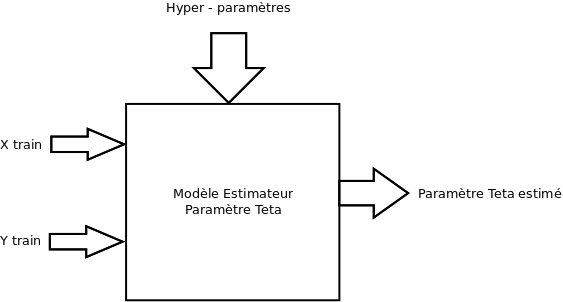
\includegraphics[scale = 0.25]{images/Diagramme1}
  		\caption{Représentation de la phase d'apprentissage.}
  		\label{fig:Apprentissage_Machine}
\end{figure}
  	
\begin{figure}[h]
 		\centering
 		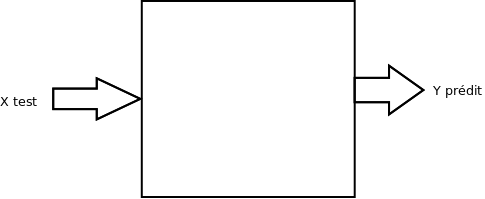
\includegraphics[scale = 0.25]{images/App_Mach_Prediction}
 		\caption{Utilisation d'un algorithme pour la prédiction de nouvelles données.}
 		\label{fig:Apprentissage_Machine_Prediction}
\end{figure}

Le critère utilisé pour choisir les paramètres lors de la phase d'apprentissage est le critère qui permet de faire le nombre d'erreurs de classification
le plus petit possible lors de la phase de test (bien qu'on n'ait pas encore les données de test).

\subsection{Sur-apprentissage \& pénalités}

Il peut arriver qu'un algorithme donne de très bons résultats sur l'ensemble d'apprentissage mais de très mauvais résultats sur l'ensemble de test.
Ce phénomène, appelé sur-apprentissage (ou apprentissage par cœur), doit être évité.

Un des moyens pour cela est d'introduire des contraintes (ou pénalités) sur les paramètres.
Il existe deux types généraux de contraintes:
\begin{itemize}
 \item les contraintes de parcimonie qui tendent à utiliser le moins de variables descriptives possibles pour la prédiction; ceci est en général réalisé en contraignant la norme $\ell_1$ du vecteur de poids
 \item les contraintes de structure qui exploitent les relations entre les variables; ceci peut être réalisé en utilisant des normes tenant compte de la structure des données comme par exemple la norme Total Variation (TV) pour les images
\end{itemize}
